%
% LaTeX Thesis Control File
%
\documentclass [11pt, proquest]{uwthesis}[2014/11/13]

%
% Custom Packages
%
\usepackage{hyperref}
\usepackage{listings}
\usepackage{xcolor}

%
% Custom Commands
%
\newcommand\todo[1]{\textcolor{red}{*ToDo: #1}}
\newcommand\ket[1]{\left|{#1}\right\rangle}
\newcommand\bra[1]{\left\langle{#1}\right|}
\newcommand\braket[2]{\left\langle{#1}|{#2}\right\rangle}

%
% Document Composition
%
\begin{document}

%
% Preliminary Pages
%
\prelimpages
%
% Copyright and Title
%
\Title{Resources Estimation for Quantum Computing Algorithms in Multiple Physical Platforms}
\Author{Cesar Zaragoza Cortes}
\Year{2021}
\Program{Physics}
\Degree{Master of Science}

\Chair{Jeffrey Wilkes}{Professor Emeritus}{Department of Physics}
\Signature{Boris Blinov}

\copyrightpage

\titlepage

%
% Abstract
%
\setcounter{page}{-1}
\abstract{%
An important task in the development of quantum computing technologies is to determine the resources needed to execute a particular algorithm in a device with certain characteristics. Resources estimation allows not only to determine whether it is possible to execute an algorithm in a current Noisy Intermediate-Scale Quantum (NISQ) device, but also to experiment with the parameters of quantum hardware to find out how much it would have to scale to achieve quantum advantage. We use the Q\# quantum programming language to implement the Bernstein-Vazirani algorithm, leverage simulators to perform resources estimation for trapped-ion and superconducting quantum hardware platforms, and compare the results.
}

%
% Contents
%
\tableofcontents
%\listoffigures % No figures yet.
%\listoftables % No tables yet.


%
% Text Pages
%
\textpages
%
% Chapter 1
%
\chapter {Introduction}

Algorithms designed for quantum computers have the potential to solve some problems that cannot be efficiently solved by algorithms designed for classical computers. However, estimating how much resources are needed to execute a quantum algorithm that outperforms a classical one is a difficult task. There are many quantum programming languages and tools built around them such as Q\#\cite{QSharp_Svore_2018}, Qiskit\cite{Qiskit_2021} and Cirq\cite{Cirq_2021} that allow execution of quantum algorithms on simulators but out-of-the-box options to estimate resources are limited to the logical level or not existent.

\section{The Purpose of This Thesis}

This thesis aims to estimate the resources required at the physical level to run Shor's semiprime integer factorization algorithm for trapped-ion and superconducting quantum hardware platforms. To do this, we will extend the simulators infrastructure built around Q\# to calculate the maximum number of physical qubits, the total number of physical gates, and the maximum runtime required to execute a particular quantum algorithm. 

Furthermore, we will also analyze the effects of errors introduced by the physical gates, analyze the feasibility of obtaining reliable results without implementing fault-tolerance, and estimate the cost of running the algorithm using error-corrected qubits and fault-tolerant gates.

In order to make this thesis more accesible to people from different backgrounds, we dedicate the next few chapters to provide a brief overview of the basics of quantum computing, quantum error correction, and Shor's semiprime integer factorization algorithm.

%
% Chapter 2
%
\chapter {Basics of Quantum Computing}

\section{Dirac Notation}

Also known as bra-ket notation, Dirac notation provides a convenient way of expressing the vectors used in quantum mechanics.

Dirac notation defines two elements:

\begin{itemize}
    \item The \textit{ket} ($\ket{\psi}$), which denotes a column vector in a complex vector space that represents a quantum state.
    $$\ket{\psi}=\left[\begin{array}{c}\psi_{1} \\ \psi_{2} \\ \cdots \\ \psi_{n} \end{array}\right]$$
    \item The \textit{bra} ($\bra{\psi}$), which denotes a row vector that is the conjugate transpose, or adjoint, of a corresponding \textit{ket} ($\ket{v}$).
    $$\bra{\psi}=\left[\begin{array}{cccc}\psi_{1}^{*} & \psi_{2}^{*} & \cdots & \psi_{n}^{*}\end{array}\right]=\left[\begin{array}{c}\psi_{1} \\ \psi_{2} \\ \cdots \\ \psi_{n} \end{array}\right]^{\dagger}$$
\end{itemize}

An \textit{operator} $\bf{A}$, represented by a $n \times n$ matrix, acting on a \textit{ket} $\ket{\psi}$ produces another \textit{ket} $\ket{\psi'}$ such that the produced \textit{ket} can be computed by matrix multiplication:
$$\ket{\psi'}=\textbf{A}\ket{\psi}=\left[\begin{array}{cc}A_{11} & A_{12} \\ A_{21} & A_{22}\end{array}\right]\left[\begin{array}{c}\psi_{1} \\ \psi_{2}\end{array}\right]=\left[\begin{array}{c}A_{11}\psi_{1}+A_{12}\psi_{2} \\ A_{21}\psi_{1}+A_{22}\psi_{2}\end{array}\right]$$

The \textit{inner product} is denoted as a bra-ket pair $\braket{\phi}{\psi}$ and represents the probability amplitude that a quantum state $\psi$ would be subsequently found in state $\phi$:
$$\braket{\phi}{\psi}=\left[\begin{array}{cc}\phi_{1}^{*} & \phi_{2}^{*} \end{array}\right]\left[\begin{array}{c}\psi_{1} \\ \psi_{2} \end{array}\right]=\phi_{1}^{*}\psi_{1}+\phi_{2}^{*}\psi_{2}$$

This notation also provides a way to describe the state vector of $n$ uncorrelated quantum states, the \textit{tensor product}:
$$\ket{\phi}\otimes\ket{\psi}=\ket{\phi}\ket{\psi}=\ket{\phi\psi}=\left[\begin{array}{c}\phi_{1} \\ \phi_{2}\end{array}\right]\otimes\left[\begin{array}{c}\psi_{1} \\ \psi_{2}\end{array}\right]=\left[\begin{array}{c}\phi_{1}\psi_{1} \\ \phi_{1}\psi_{2} \\ \phi_{2}\psi_{1} \\ \phi_{2}\psi_{2}\end{array}\right]$$

Note that $\ket{\psi}^{\otimes n}$ represents the tensor product of $n$ $\ket{\psi}$ quantum states:
$$\ket{\psi}^{\otimes n}=\ket{\psi}\otimes\cdots\otimes\ket{\psi}=\ket{\psi}\cdots\ket{\psi}=\ket{\psi\cdots\psi}=\left[\begin{array}{c}\psi_{1} \\ \psi_{2} \end{array}\right]\otimes\cdots\otimes\left[\begin{array}{c}\psi_{1} \\ \psi_{2} \end{array}\right]$$

\section{Quantum Systems}

Quantum mechanics is a mathematical framework for the development of physical theories\cite{NielsenChuang_2012}. On its own quantum mechanics doesn't tell you what laws a physical system must obey, but it does provide a mathematical and conceptual framework for the development of such laws. The postulates described next provide a connection between the physical world and the mathematical formalism of quantum mechanics.

Postulate 1: The state of an isolated physical system is fully described by a unit vector $\ket{\psi}$ in Hilbert space.

Postulate 2: The evolution of a closed quantum system is described by a unitary transformation. This means that the state $\ket{\psi}$ at time $t_1$ is related to the state $\ket{\psi'}$ at time $t_2$ by a unitary operator $U$ which depends only on the times $t_1$ and $t_2$:

$$\ket{\psi'}=U(t_1,t_2)\ket{\psi}$$

Postulate 3: The state space of a composite physical system is the tensor product of the state spaces of the component physical systems.

Postulate 4: Quantum measurements are described by a collection of ${M_m}$ of measurement operators.

\section{Qubits}

In classical information theory and classical computing, a bit is the fundamental building block.
Analogously, in quantum information theory and quantum computing, a quantum bit or qubit is the fundamental building block.

Physically, a quibit is a two-level quantum-mechanical system. The polarization of a single photon and the spin of the electron are examples of such systems.

Mathematically, a qubit is a linear combination of states $\ket{\psi}=\alpha\ket{0}+\beta\ket{1}$ where $\alpha$ and $\beta$ are complex numbers known as amplitudes, and $\ket{0}$ and $\ket{1}$ are the computational basis states.

When a qubit is measured, the result is either $\ket{0}$ with probability $|\alpha|^2$ or $\ket{1}$ with probability $|\beta|^2$.
Since the probabilities must sum to one, the qubit's state is normalized:
$$|\alpha|^2+|\beta|^2=1$$

The computational basis states, which are analogous to the two values ($0$ and $1$) that a classical bit may take, form an orthonormal basis represented by the following vectors:
$$\ket{0}=\left[\begin{array}{c}1 \\ 0\end{array}\right]$$
$$\ket{1}=\left[\begin{array}{c}0 \\ 1\end{array}\right]$$

Using the previous definitions, we can see a qubit as a unit vector in two-dimensional complex vector space:
\[\ket{\psi}=\left[\begin{array}{c}\alpha \\ \beta\end{array}\right]\]

\section{Superposition}

The principle of quantum superposition states that the most general state of a quantum-mechanical system is a linear combination of all distinct valid quantum states. A qubit is an example of a quantum superposition of the basis states $\ket{0}$ and $\ket{1}$.

A concrete example of a qubit in superposition that has the same probability of being measured as $\ket{0}$ or $\ket{1}$ is the following:
$$\ket{\psi}=\frac{1}{\sqrt{2}}\left(\ket{0}+\ket{1}\right)$$

\section{Quantum Logic Gates}

In classical digital circuits, logic gates are the building blocks. Analogously, in the quantum circuit model of computation, quantum logic gates are the building blocks of quantum algorithms. Quantum gates act on qubits, transform them in different ways, and can be applied sequentially to perform complex quantum computations.

Quantum gates are unitary operators represented as $2^n \times 2^n$ unitary matrices where $n$ is the number of qubits the gate operates on. Unitary matrices are complex square matrices $\bf{U}$ which have the property that its conjugate transpose or adjoint $\bf{U^{\dagger}}$ is also its inverse $\bf{U^{-1}}$:
$$\bf{U^{\dagger}U}=\bf{UU^{\dagger}}=\bf{UU^{-1}}=I$$

A quantum gate is applied to a qubit system by multiplying the gate's matrix representation by the qubits' state vector. This operation transforms the qubit system:
$$\ket{\psi_1}=\bf{U}\ket{\psi_0}$$

Applying a sequence of quantum gates is equivalent to performing a series of these multiplications. For example, applying gate $\bf{U_a}$ followed by a gate $\bf{U_b}$ to a state vector $\ket{\psi}$ is represented by the follwing expression where the gates closest to the state vector are applied first:
$$\bf{U_b}\bf{U_a}\ket{\psi}$$

Since matrix multiplication is associative, multiplying $\bf{U_a}$ by $\bf{U_b}$ produces a compund gate $\bf{U_{b}U_{a}}$ that is equivalent to applying $\bf{U_a}$ followed by $\bf{U_b}$:
$$\bf{U_b}\bf{U_a}\ket{\psi}=\bf{U_b}(\bf{U_a}\ket{\psi})=(\bf{U_b}\bf{U_a})\ket{\psi}$$

Note that all quantum gates are reversible since they are represented by unitary matrices. This means that for any gate, another gate exists that reverts the gate's transformation on a state vector:
$$\ket{\psi}=\bf{U^{\dagger}}(\bf{U}\ket{\psi})=\bf{U^{\dagger}}\bf{U}\ket{\psi}=\bf{I}\ket{\psi}$$

\section{Single-Qubit Gates}

Single-qubit gates are represented by $2 \times 2$ unitary matrices. Applying a gate to a matrix can be done by multiplying the gate's matrix by the qubit's state vector.

Next, some of the most commonly used gates.

Pauli-X gate:
$$X=\left[\begin{array}{cc}0 & 1 \\ 1 & 0\end{array}\right]$$

Pauli-Y gate:
$$Y=\left[\begin{array}{cc}0 & -\imath \\ \imath & 0\end{array}\right]$$

Pauli-Z gate:
$$Z=\left[\begin{array}{cc}1 & 0 \\ 0 & -1\end{array}\right]$$

Hadamard gate:
$$H=\frac{1}{\sqrt{2}}\left[\begin{array}{cc}1 & 1 \\ 1 & -1\end{array}\right]$$

RX gate:
$$R_x(\theta)=\left[\begin{array}{cc}cos{\frac{\theta}{2}} & -\imath sin{\frac{\theta}{2}} \\ -\imath sin{\frac{\theta}{2}} & cos{\frac{\theta}{2}}\end{array}\right]$$

RY gate:
$$R_y(\theta)=\left[\begin{array}{cc}cos{\frac{\theta}{2}} & -sin{\frac{\theta}{2}} \\ sin{\frac{\theta}{2}} & cos{\frac{\theta}{2}}\end{array}\right]$$

RZ gate:
$$R_z(\theta)=\left[\begin{array}{cc}e^{-\imath \frac{\theta}{2}} & 0 \\ 0 & e^{\imath \frac{\theta}{2}}\end{array}\right]$$

R1 gate:
$$R_1(\theta)=\left[\begin{array}{cc}1 & 0 \\ 0 & e^{\imath \theta}\end{array}\right]$$

\section{Multi-Qubit Gates}

Multi-qubit gates are represented by $2^N \times 2^N$ matrices where N is the number of qubits the gate operates on.

Of special importance is the CNOT gate which is a two-qubit gate where the first qubit is referred to as the control qubit and the second qubit as the target qubit. CNOT acts as a conditional gate, if the control qubit is in state $\ket{1}$, it applies the Pauli X gate to the target qubit, otherwise it does nothing. The main use of this gate is to prepare entangled states.

$$CNOT=\left[\begin{array}{cccc}1 & 0 & 0 & 0 \\ 0 & 1 & 0 & 0 \\ 0 & 0 & 0 & 1 \\ 0 & 0 & 1 & 0\end{array}\right]$$

%
% Chapter 3
%
\chapter {Basics of Quantum Error Correction}

This chapter explains the basic concepts to understand how quantum computations can be performed reliably in the presence of noise. Given the fragility of coherent quantum systems, quantum error correction and fault-tolerant quantum computation are fundamental arbitrarily large quantum algorithms operating on many qubits.

\section{Noise and Error Correction}

Noise can introduce errors in data while it is being processed, sent through a channel and/or stored in a medium. A common error that can be introduced by noise is a bit flip (e.g. $0 \rightarrow 1$, $1 \rightarrow 0$). The task of error correction is to detect when an error has occurred and correct it.

In classical error correction, coding based on data-copying is extensively used. The key idea is to protect data against the effects of noise by adding redundancy. For example, a classical repetition code can encode a logical bit using three physical bits:
$$0 \rightarrow 000$$
$$1 \rightarrow 111$$

The problem is that classical error correction techniques cannot be directly applied to qubits because of the following reasons:
\begin{itemize}[noitemsep]
    \item It is impossible to create an independent and identical copy of a qubit in an arbitrary unknown state. This is known as the no-cloning theorem of quantum mechanics and it has the consequence that qubits cannot be protected from errors by simply making multiple copies\cite{NoCloningTheorem_1982}.
    \item Measurement destroys quantum information, implying that we cannot measure a qubit to decide which correcting action to perform.
    \item In addition to bit flip errors ($\ket{\psi}=\alpha\ket{0}+\beta\ket{1} \rightarrow \ket{\psi}=\alpha\ket{1}+\beta\ket{0}$), qubits are also susceptible to phase flip errors ($\ket{\psi}=\alpha\ket{0}+\beta\ket{1} \rightarrow \ket{\psi}=\alpha\ket{0}-\beta\ket{1}$) that have no classical analogous. Therefore, quantum error correction must be able to simultaneously correct for both.
    \item Errors in quantum information are continuous. This means that qubits, in the presence of noise, experience angular shifts rather than full bit or phase flips.
\end{itemize}

In order to protect qubits against the effects of noise, we can use the following process:
\begin{enumerate}[noitemsep]
    \item Encode: multiple physical qubits are used to encode a two-level quantum state into a logical qubit.
    \item Manipulation: operations are performed using the logical qubit (here's where errors can be introduced).
    \item Syndrome detection: measurements are performed that indicate what error, if any, ocurred.
    \item Recovery: the value of the syndrome is used to select the procedure to use to correct the error.
    \item Decode: logical qubit is decoded before final measurements are made.
\end{enumerate}

\section{Bit Flip Code}

To make it possible to correct bit flip errors, we can use three physical qubits to encode each logical qubit:
$$\ket{0_L}=\ket{000}$$
$$\ket{1_L}=\ket{111}$$
$$\ket{\psi}=\alpha\ket{0}+\beta\ket{1}  \underrightarrow{encode}  \ket{{\psi}_{L}}=\alpha\ket{0_L}+\beta\ket{1_L}$$

The notation $\ket{0_L}$ and $\ket{1_L}$ indicates that these are the logical $\ket{0}$ and logical $\ket{1}$ states, and not the physical $\ket{0}$ and physical $\ket{1}$ states.

A circuit that performs this encoding is illustrated in figure \ref{fig:BitFlipEncodingCircuit}:

\begin{figure}[h!]
    \centering
    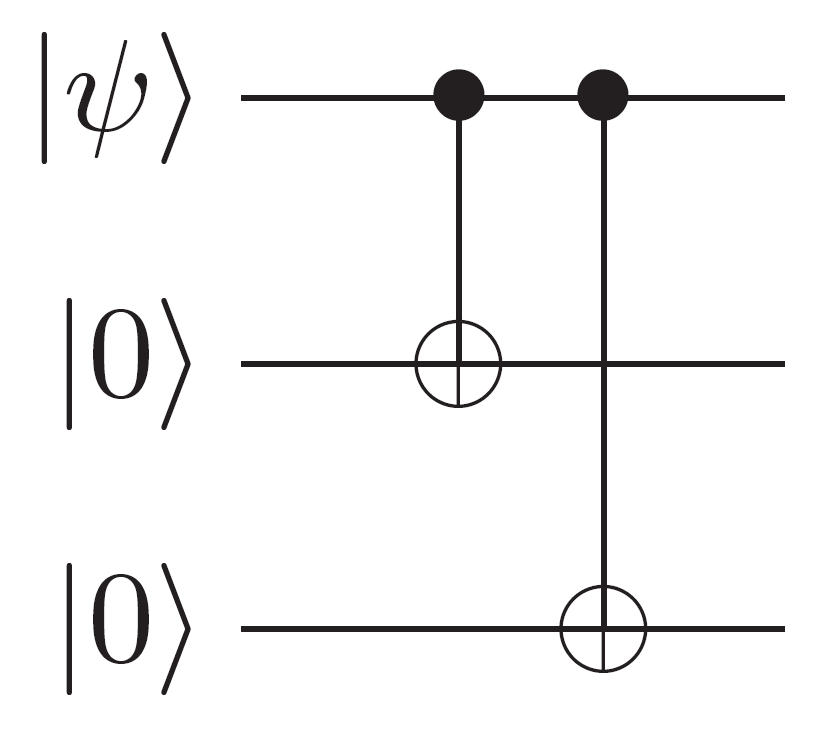
\includegraphics[scale=.25]{images/ErrorCorrection-BitFlipEncodingCircuit.png}
    \caption{Bit flip encoding circuit \cite{NielsenChuang_2012}}
    \label{fig:BitFlipEncodingCircuit}
\end{figure}

After the logical qubit has been manipulated, syndrome detection and recovery is done. There are four bit flip posibilities at this stage:
\begin{itemize}[noitemsep]
    \item No error: $\alpha\ket{000}+\beta\ket{111}$
    \item First qubit flipped: $\alpha\ket{100}+\beta\ket{011}$
    \item Second qubit flipped: $\alpha\ket{010}+\beta\ket{101}$
    \item Third qubit flipped: $\alpha\ket{001}+\beta\ket{110}$
\end{itemize}

For each one of these posibilities, the recovery operation is clear. The circuit shown in figure \ref{fig:BitFlipDetectionAndRecoveryCircuit} detects the error using two auxiliary qubits that are entangled with the logical qubit such that measurements on those qubits yield two classical bits of information whose values map to a specific recovery operation that is then applied. Note that the $X$ gate is used as the recovery operation.

\begin{figure}[h!]
    \centering
    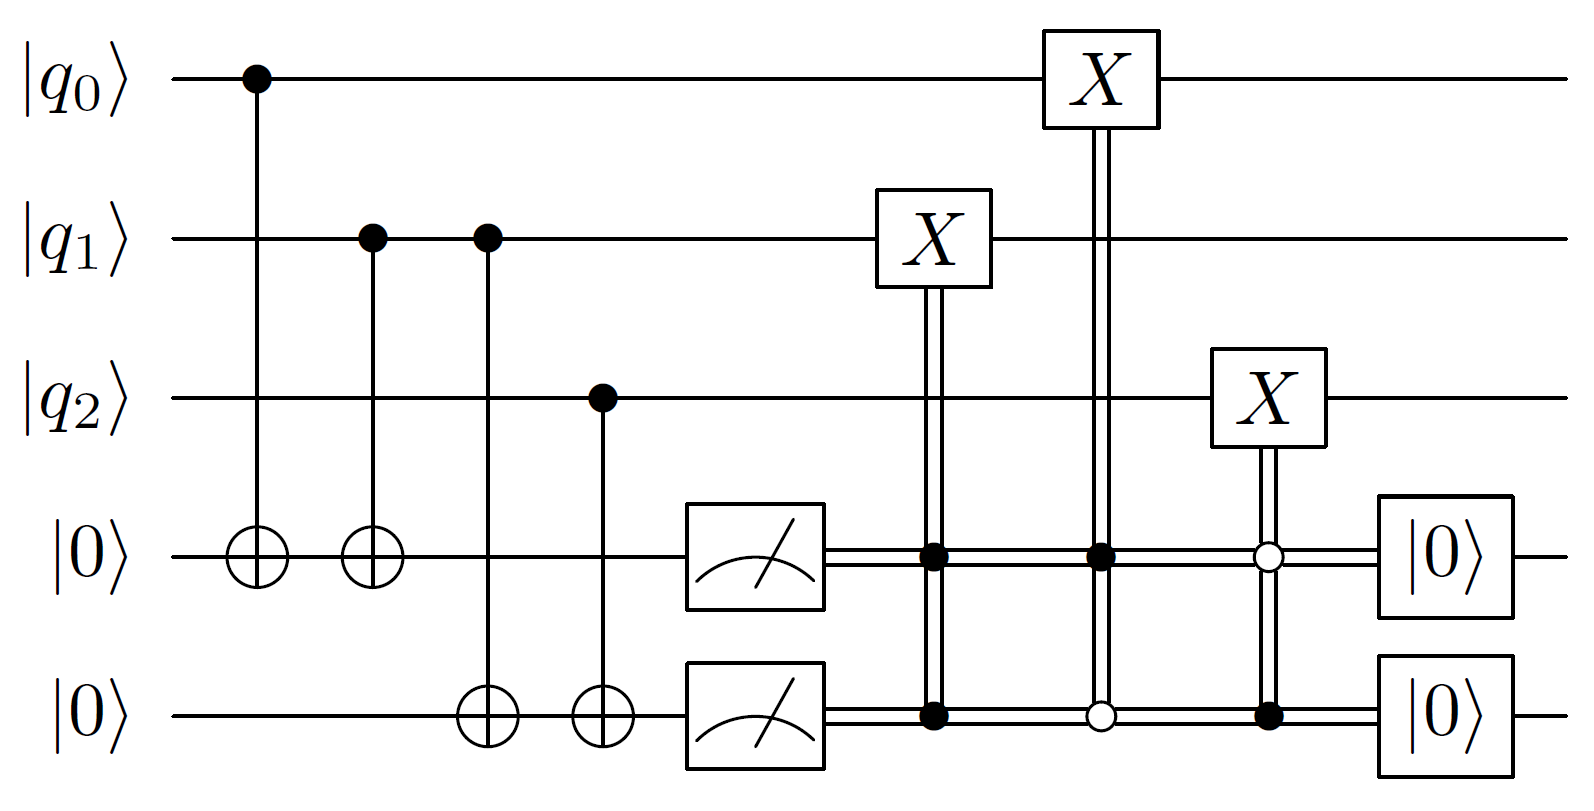
\includegraphics[scale=.25]{images/ErrorCorrection-BitFlipDetectionAndRecoveryCircuit.png}
    \caption{Bit flip detection and recovery circuit \cite{ThomasWong_2022}}
    \label{fig:BitFlipDetectionAndRecoveryCircuit}
\end{figure}

\section{Phase Flip Code}

Phase flip errors can similarly be corrected by using three physical qubits to encode a logical qubit. Since a complete phase flip error in the $\ket{+}$ and $\ket{-}$ basis switches between these states, logical qubits are the following:
$$\ket{0_L}=\ket{+++}$$
$$\ket{1_L}=\ket{---}$$
$$\ket{\psi}=\alpha\ket{0}+\beta\ket{1}  \underrightarrow{encode}  \ket{{\psi}_{L}}=\alpha\ket{0_L}+\beta\ket{1_L}$$

A circuit that performs this encoding is illustrated in figure \ref{fig:PhaseFlipEncodingCircuit}:

\begin{figure}[h!]
    \centering
    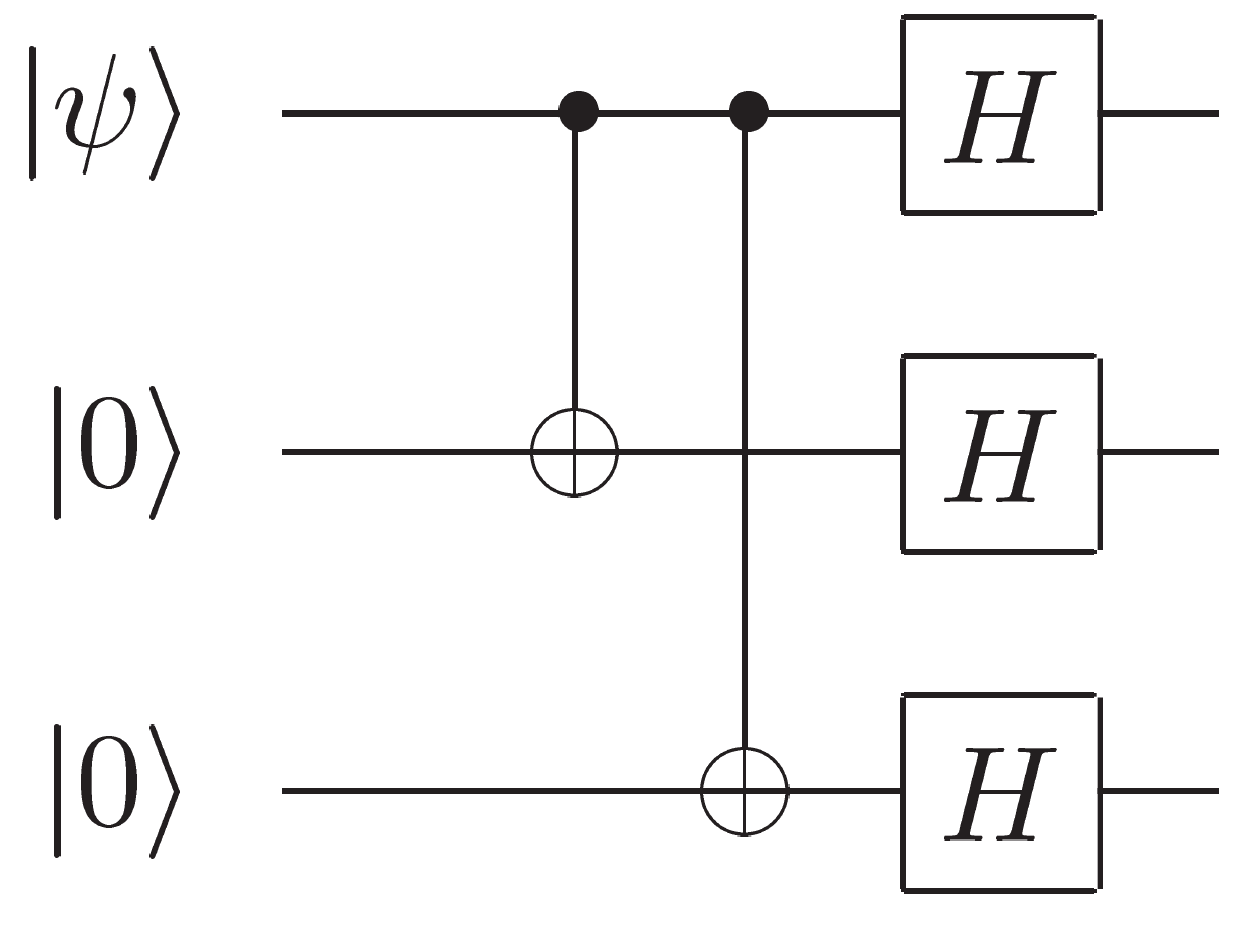
\includegraphics[scale=.25]{images/ErrorCorrection-PhaseFlipEncodingCircuit.png}
    \caption{Phase flip encoding circuit \cite{NielsenChuang_2012}}
    \label{fig:PhaseFlipEncodingCircuit}
\end{figure}

After the logical qubit has been manipulated, syndrome detection and recovery is done. Like in the bit flip case, there are four posibilities at this stage:
\begin{itemize}[noitemsep]
    \item No error: $\alpha\ket{+++}+\beta\ket{---}$
    \item First qubit flipped: $\alpha\ket{-++}+\beta\ket{+--}$
    \item Second qubit flipped: $\alpha\ket{+-+}+\beta\ket{-+-}$
    \item Third qubit flipped: $\alpha\ket{++-}+\beta\ket{--+}$
\end{itemize}

The circuit shown in figure \ref{fig:PhaseFlipDetectionAndRecoveryCircuit} detects the error using two auxiliary qubits that are entangled with the logical qubit such that measurements on those qubits yield two classical bits of information whose values map to a specific recovery operation that is then applied. In this case, instead of using the $X$ gate to correct errors, the $Z$ gate is used as the recovery operation for the qubit that was flipped.

\begin{figure}[h!]
    \centering
    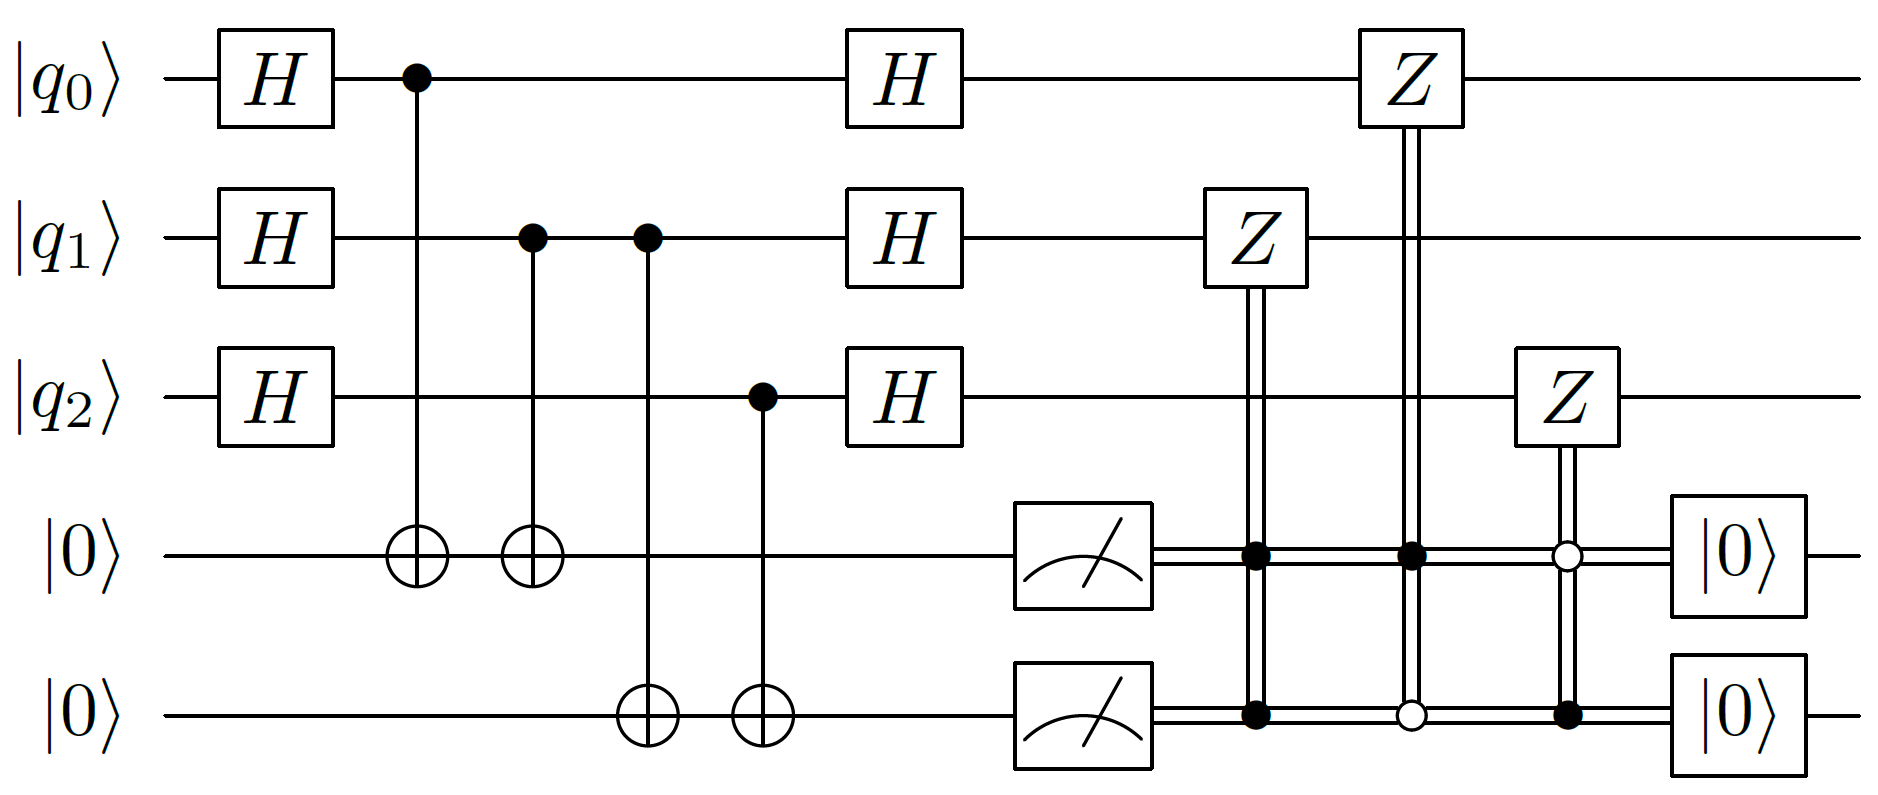
\includegraphics[scale=.25]{images/ErrorCorrection-PhaseFlipDetectionAndRecoveryCircuit.png}
    \caption{Bit flip detection and recovery circuit \cite{ThomasWong_2022}}
    \label{fig:PhaseFlipDetectionAndRecoveryCircuit}
\end{figure}

\section{Shor Code}

There is a quantum code which can protect against the effects of an arbitrary error on a single qubit knwon as the Shor code. The code is a combination of three qubit phase flip and bit flip codes. First, we encode the qubit using the phase flip code such that $\ket{0} \rightarrow \ket{+++}$ and $\ket{1} \rightarrow \ket{---}$. Next, we encode each one of these qubits using the three qubit bit flip code such that $\ket{+} \rightarrow \frac{\ket{000}+\ket{111}}{\sqrt{2}}$ and $\ket{-} \rightarrow \frac{\ket{000}-\ket{111}}{\sqrt{2}}$. This results in the following logical qubits:
$$\ket{0_L}=\frac{(\ket{000}+\ket{111})(\ket{000}+\ket{111})(\ket{000}+\ket{111})}{2\sqrt{2}}$$
$$\ket{1_L}=\frac{(\ket{000}-\ket{111})(\ket{000}-\ket{111})(\ket{000}-\ket{111})}{2\sqrt{2}}$$

A circuit that performs this encoding is illustrated in figure \ref{fig:ShorEncodingCircuit}:

\begin{figure}[h!]
    \centering
    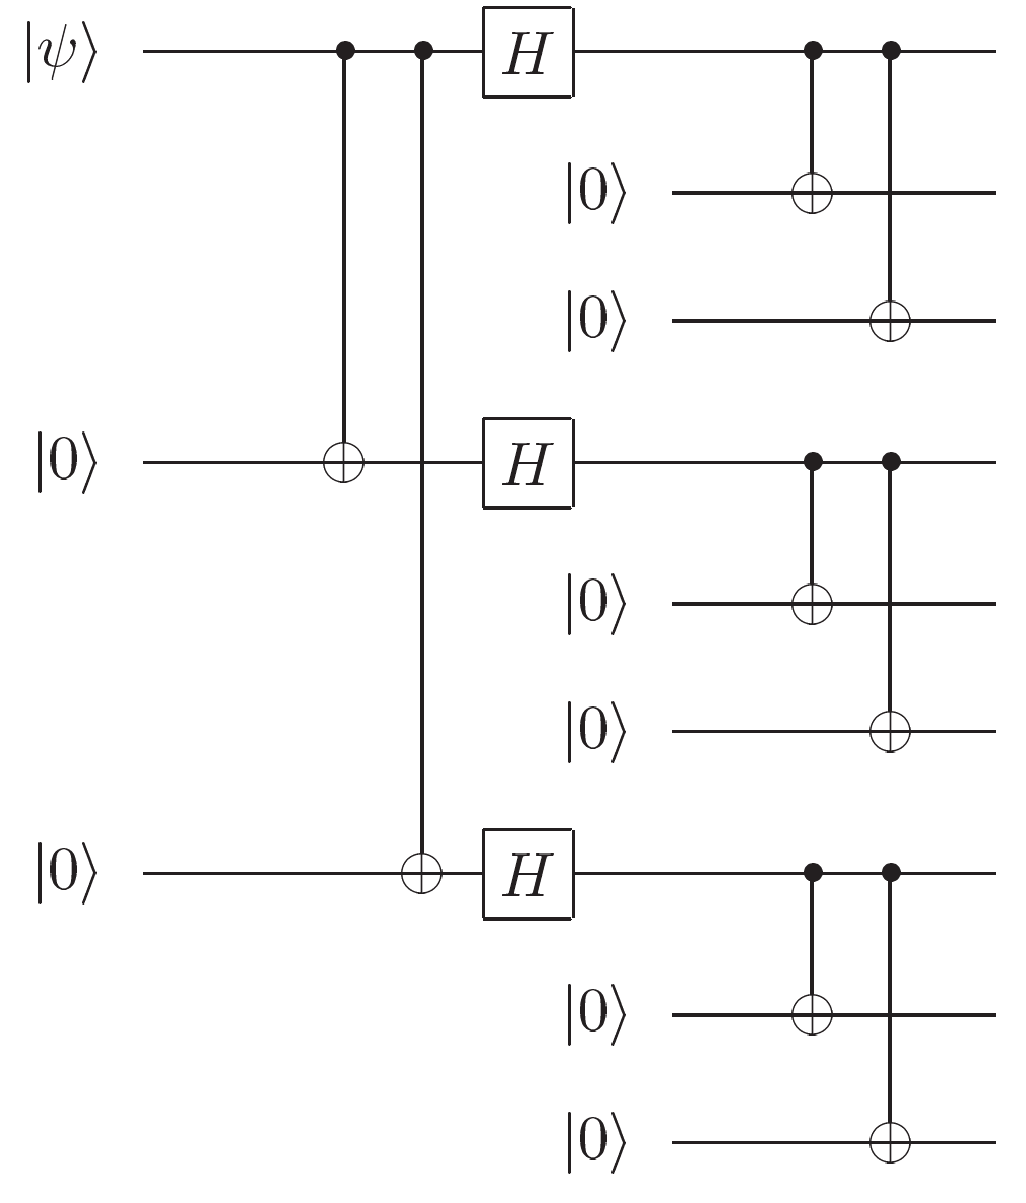
\includegraphics[scale=.25]{images/ErrorCorrection-ShorEncodingCircuit.png}
    \caption{Phase flip encoding circuit \cite{NielsenChuang_2012}}
    \label{fig:ShorEncodingCircuit}
\end{figure}

Syndrome detection and recovery for the Shor code is performed by combining bit flip and phase flip detection and recovery. Figure \ref{fig:ShorBitFlipDetectionAndRecoveryCircuit} shows bit flip detection and recovery. To do the same for phase flips we would just have to use the previously shown phase flip detection and recovery circuit on the first qubit of each bit flip encoded block.

\begin{figure}[h!]
    \centering
    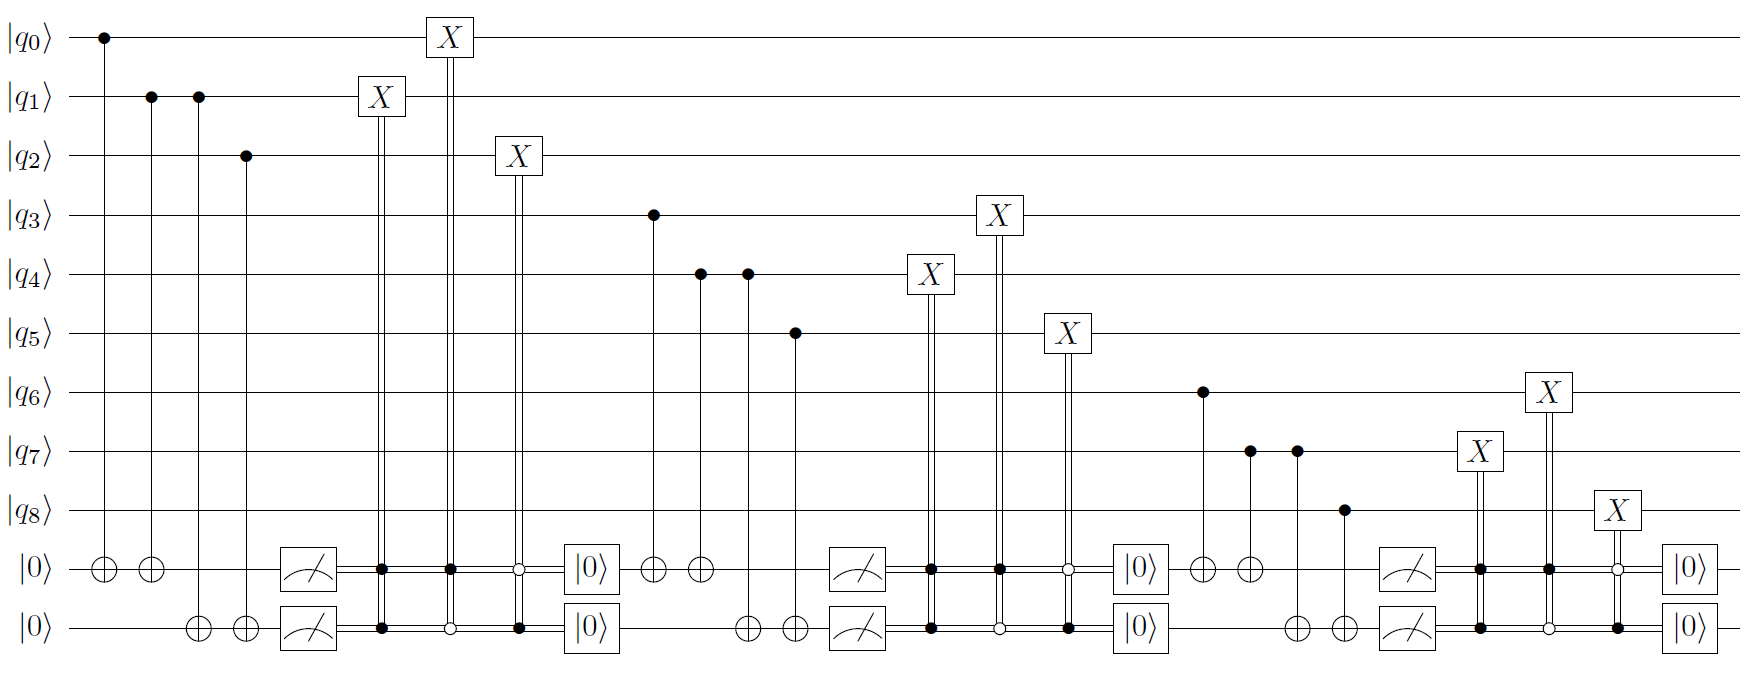
\includegraphics[scale=.35]{images/ErrorCorrection-ShorBitFlipDetectionAndRecoveryCircuit.png}
    \caption{Bit flip detection and recovery circuit on a Shor encoded qubit \cite{ThomasWong_2022}}
    \label{fig:ShorBitFlipDetectionAndRecoveryCircuit}
\end{figure}

Note that the Shor code corrects all quantum errors assuming each triplet experiences at most one bit flip error per correction cycle, and at most one triplet experiences a phase flip error per correction cycle.

\section{Quantum Error-Correction Without Measurement}

We have described quantum error-correction as a two stage process: a syndrome detection step that uses quantum measurement followed by a recovery step that applies unitary operations based on the results of the measurement. It is posible to perform error-correction using only unitary operations and auxiliary qubits prepared in standard states.

For example, figure \ref{fig:BitFlipDetectionAndRecoveryCircuitDelayedMeasurement} shows a delayed measurement circuits that perform syndrome detection and error recovery for bit flip errors:

\begin{figure}[h!]
    \centering
    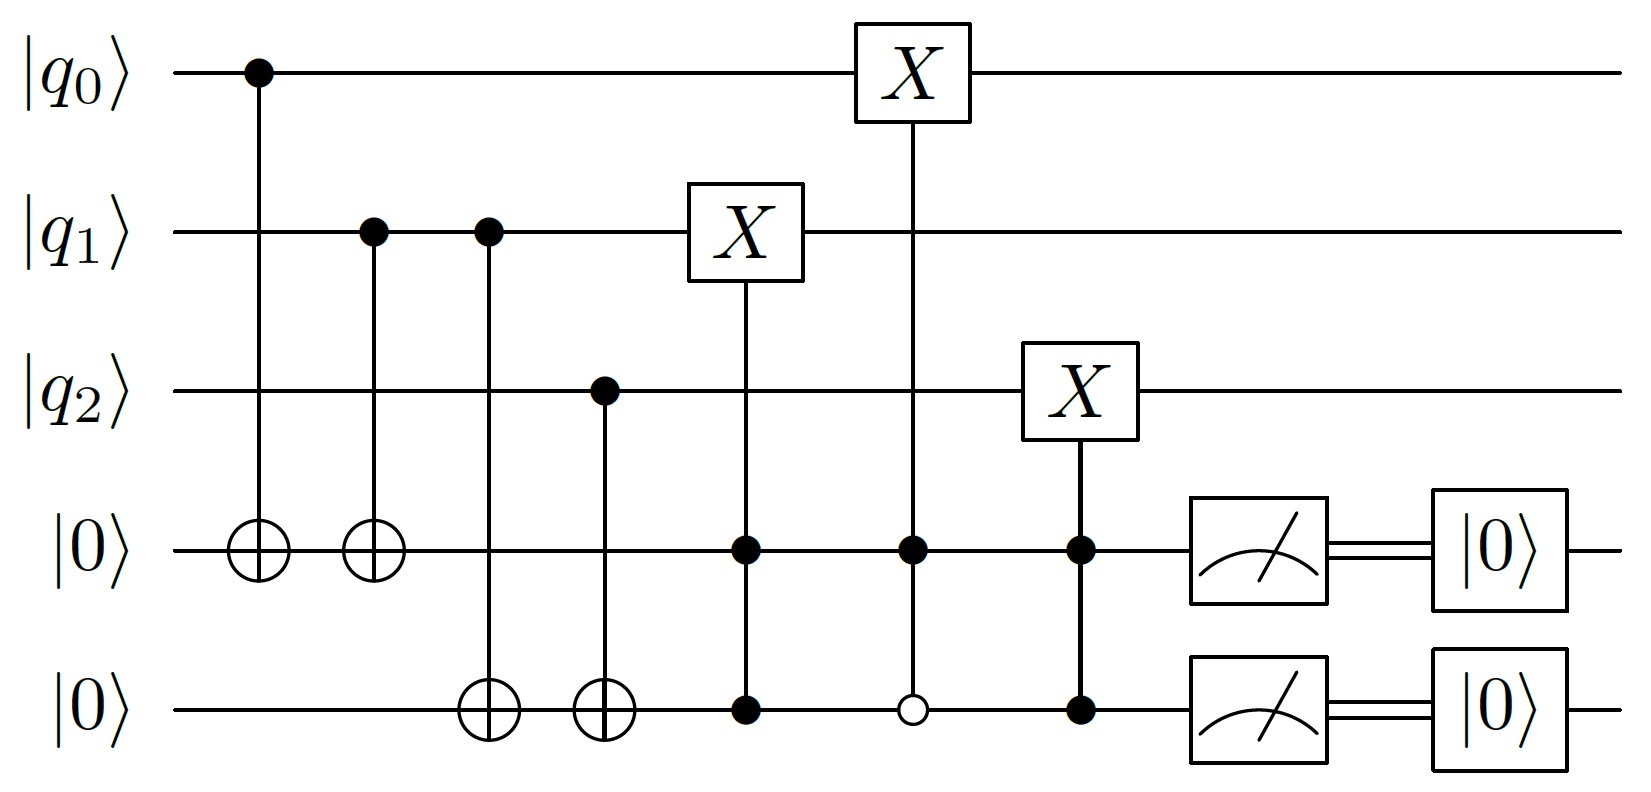
\includegraphics[scale=.25]{images/ErrorCorrection-BitFlipDetectionAndRecoveryCircuitDelayedMeasurement.png}
    \caption{Bit flip detection and recovery circuit using delayed measurement \cite{ThomasWong_2022}}
    \label{fig:BitFlipDetectionAndRecoveryCircuitDelayedMeasurement}
\end{figure}

The advantage this provides is that for some real-world quantum systems it is very difficult to apply different unitary operations based on quantum measurements so an alternate procedure is needed.

\section{Fault-Tolerant Quantum Computation}

One of the most useful applications of quantum error correction is the protection of quantum information as it dynamically undergoes computation. An arbitrary good quantum computation can be achieved provided only that the error probability per gate is below a certain constant threshold. A quantum computer that accumulates error slow enough that error can be corrected in called fault-tolerant.

The basic idea behind fault-tolerant quantum computation is to perform computations directly on encoded logical qubits such that decoding is never required.

Figure \ref{fig:FaultTolerantCircuit} shows a circuit using fault-tolerant logical operations. In this specific case, seven physical qubits are being used to encode and error-correct each logical qubit. One thing to note is that the reason the second error-correction step performed in the second qubit is that simply storing qubits for a period of time introduces errors and should periodically be error-corrected in order to prevent acumulation of errors.

\begin{figure}[h!]
    \centering
    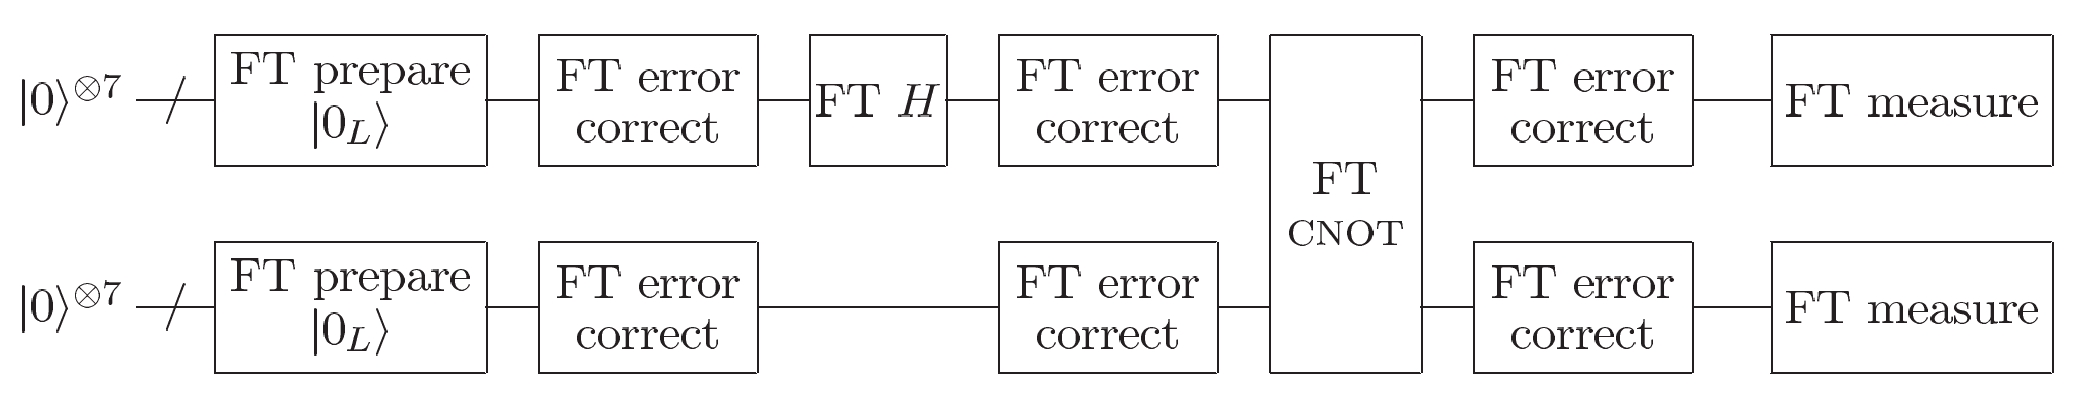
\includegraphics[scale=.30]{images/ErrorCorrection-FaultTolerantCircuit.png}
    \caption{Example of a fault-tolerant circuit \cite{NielsenChuang_2012}}
    \label{fig:FaultTolerantCircuit}
\end{figure}

%
% Chapter 4
%
\chapter {Shor's Semiprime Integer Factorization Algorithm}

Shor's algorithm is a polynomial-time quantum algorithm for semiprime integer factorization. In comparison, the time complexity of the most efficient known classical factoring algorithm is superpolynomial.

We chose Shor's algorithm because it is one of the most significant quantum algorithms, and because the number of qubits and the number of quantum operations required are proportional to the input size. The number of operations is particullarly relevant since it makes the errors introduced by the physical gates an important consideration.

\section{Algorithm}

The problem that Shor's algorithm solves is the following: given a semiprime integer \textit{N}, find its two prime factor \textit{p} and \textit{q}.

Shor's algorithm combines both classical and quantum computations, and the procedure to perform it is the following:
\begin{enumerate}
    \item Pick a random integer $1 < a < N$.
    \item Check whether $a$ is a factor by determining whether $a$ and $N$ are comprime. If they are, we can compute the factors. Otherwise continue with the rest of the algorithm.
    \item Use a period-finding quantum subroutine to find the period $r$ of the function $f(x)=a^{x} \ mod \ N$.
    \item If $r$ is odd, then go back to step 1. If $r$ is even, go to the next step.
    \item If $a^{\frac{r}{2}} \equiv -1  \ mod \ N$, then go back to step 1.
    \item Either $a^{\frac{r}{2}} - 1$ or $a^{\frac{r}{2}} + 1$ shares a factor with $N$.
\end{enumerate}

\section{Q\# Implementation}

In order to take advantage of the tools built around Q\#, we use a modified implementation of Shor's algorithm found in Microsoft's quantum samples GitHub repository.

\todo{Add reference to Microsoft's quantum samples repository.}

\todo{Breakdown the implementation into different sections and describe each one (similar to what is done in the "Learn Quantum Computing with Python and Q\#" book).}

The following Q\# code presents a top-level implementation of Shor's algorithm.

\begin{lstlisting}[language=C]
@EntryPoint()
operation FactorSemiprimeInteger(N : Int) : (Int, Int) {

    // Check the most trivial case where N is pair.
    if (N % 2 == 0) {
        return (2, N / 2);
    }

    mutable factors = (1, 1);
    mutable foundFactors = false;
    repeat {

        // Start by guessing a coprime to N.
        let coprimeGuess = DrawRandomInt(1, N - 1);

        // If the guess number is a coprime, use a quantum algorithm for period finding.
        // Otherwise, the GCD between N and the coprime guess number is one of the factors.
        if (IsCoprimeI(N, coprimeGuess)) {
            let period = EstimatePeriod(N, coprimeGuess);
            set (foundFactors, factors) = CalculateFactorsFromPeriod(N, coprimeGuess, period);
        } else {
            let gcd = GreatestCommonDivisorI(N, coprimeGuess);
            set (foundFactors, factors) = (true, (gcd, N / gcd));
        }
    }
    until foundFactors

    return factors;
}
\end{lstlisting}

\section{Quantum Subroutine}

\todo{Show the circuit representation of the quantum subroutine.}

The following Q\# code implements the period finding quantum subroutine:

\begin{lstlisting}[language=C]
    @EntryPoint()
    operation EstimatePeriodInstance(N : Int, a : Int) : (Bool, Int) {
    
        // Prepare eigenstate register.
        let bitSize = BitSizeI(N);
        use eigenstateRegister = Qubit[bitSize];
        let eigenstateRegisterLE = LittleEndian(eigenstateRegister);
        ApplyXorInPlace(1, eigenstateRegisterLE);
    
        // Prepare phase register.
        let bitsPrecision =  2 * bitSize + 1;
        use phaseRegister = Qubit[bitsPrecision];
        let phaseRegisterLE = LittleEndian(phaseRegister);
    
        // Prepare oracle for quantum phase estimation.
        let oracle = DiscreteOracle(ApplyOrderFindingOracle(N, a, _, _));
    
        // Execute quantum phase estimation.
        QuantumPhaseEstimation(oracle, eigenstateRegisterLE!, LittleEndianAsBigEndian(phaseRegisterLE));
    
        let phaseEstimate = MeasureInteger(phaseRegisterLE);
    
        // Reset qubit registers 
        ResetAll(eigenstateRegister);
    
        // Return period calculation based on estimated phase.
        return CalculatePeriodFromPhaseEstimate(N, bitsPrecision, phaseEstimate);
    }
\end{lstlisting}

%
% Chapter 5
%
\chapter {Analysis Framework}

The strategy we use to analyze this algorithm is very similar to the one proposed by Soeken et al.\cite{ResourceEstimationFramework_Soeken_2021}. The process is the following:
\begin{enumerate}
    \item Implement a quantum algorithm using a high-level programming language (Q\# in this case).
    \item Verify the correctness of the implementation by executing the algorithm in a full state simulator.
    \item Use the built-in resources estimator to roughly calculate the amount of logical quantum gates used by the algorithm depending on the input size.
    \todo{This part can be done in its own chapter and that chapter can explain in detail how the built-in resources estimator works and how to interpret the data that it produces.}
    \item For each hardware platform do the following:
    \begin{enumerate}
        \item Create a resources estimator that uses hardware specific parameters to calculate the amount of physical qubits, physical gates, and runtime required to run the algorithm.
        \item Analyze data produced by the resources estimator to determine the maximum input size for the algorithm to run on a real NISQ device.
        \item Analyze data produced by the resources estimator to determine the characteristics that a device should have to run the algorithm for a specific input size, and determine what would be the runtime.
    \end{enumerate}
    \item Compare the results for each hardware platform.
\end{enumerate}

\todo{Explain the following}
\begin{itemize}
    \item Resources Metrics: Describe the values obtained from the resources estimator (gate count, runtime, accumulated error), and how they are calculated.
    \item Gate Decomposition: Describe why logical-level gates have to be decomposed into physical-level gates.
    \item Limitations: Describe the limitations that this resources estimation has in regards to runtime (sum of the runtimes of individual gates rather than the critical path), and types of computations (trouble with mixed states).
\end{itemize}

\section{Extending Q\# Simulation Infrastructure for Estimation of Physical Resources}

Microsoft's Quantum Development Kit (QDK) supports the implementation of custom simulators that can be used to run Q\# programs. We leverage this capability and implement a simulator that calculates the resources a quantum algorithm would require to be executed in a hardware platform with specific characteristics.

\todo{Explain the following}
\begin{itemize}
    \item QDK Custom Simulators: Describe how custom simulators are implemented using diagrams and code snippets.
    \item Software Architecture of Physical Resources Estimator Simulator: Describe the software architecture using diagrams and code snippets.
\end{itemize}

Source code of a working version can be found in in \href{https://github.com/cesarzc/uw-master-in-physics-project}{GitHub}.

%
% Chapter 6
%
\chapter {Shor's Algorithm Logical Analysis}

\section{Q\# Implementation}

In order to take advantage of the tools built around Q\#, we use a modified implementation of Shor's algorithm found in Microsoft's quantum samples GitHub repository.

\todo{Add reference to Microsoft's quantum samples repository.}

\todo{Breakdown the implementation into different sections and describe each one (similar to what is done in the "Learn Quantum Computing with Python and Q\#" book).}

The following Q\# code presents a top-level implementation of Shor's algorithm.

\begin{lstlisting}[language=C]
@EntryPoint()
operation FactorSemiprimeInteger(N : Int) : (Int, Int) {

    // Check the most trivial case where N is pair.
    if (N % 2 == 0) {
        return (2, N / 2);
    }

    mutable factors = (1, 1);
    mutable foundFactors = false;
    repeat {

        // Start by guessing a coprime to N.
        let coprimeGuess = DrawRandomInt(1, N - 1);

        // If the guess number is a coprime, use a quantum algorithm for period finding.
        // Otherwise, the GCD between N and the coprime guess number is one of the factors.
        if (IsCoprimeI(N, coprimeGuess)) {
            let period = EstimatePeriod(N, coprimeGuess);
            set (foundFactors, factors) = CalculateFactorsFromPeriod(N, coprimeGuess, period);
        } else {
            let gcd = GreatestCommonDivisorI(N, coprimeGuess);
            set (foundFactors, factors) = (true, (gcd, N / gcd));
        }
    }
    until foundFactors

    return factors;
}
\end{lstlisting}

\section{Quantum Subroutine}

\todo{Show the circuit representation of the quantum subroutine.}

The following Q\# code implements the period finding quantum subroutine:

\begin{lstlisting}[language=C]
    @EntryPoint()
    operation EstimatePeriodInstance(N : Int, a : Int) : (Bool, Int) {
    
        // Prepare eigenstate register.
        let bitSize = BitSizeI(N);
        use eigenstateRegister = Qubit[bitSize];
        let eigenstateRegisterLE = LittleEndian(eigenstateRegister);
        ApplyXorInPlace(1, eigenstateRegisterLE);
    
        // Prepare phase register.
        let bitsPrecision =  2 * bitSize + 1;
        use phaseRegister = Qubit[bitsPrecision];
        let phaseRegisterLE = LittleEndian(phaseRegister);
    
        // Prepare oracle for quantum phase estimation.
        let oracle = DiscreteOracle(ApplyOrderFindingOracle(N, a, _, _));
    
        // Execute quantum phase estimation.
        QuantumPhaseEstimation(oracle, eigenstateRegisterLE!, LittleEndianAsBigEndian(phaseRegisterLE));
    
        let phaseEstimate = MeasureInteger(phaseRegisterLE);
    
        // Reset qubit registers 
        ResetAll(eigenstateRegister);
    
        // Return period calculation based on estimated phase.
        return CalculatePeriodFromPhaseEstimate(N, bitsPrecision, phaseEstimate);
    }
\end{lstlisting}


\todo{Explain the following}
\begin{itemize}
    \item Resources Metrics: Describe the values obtained from the resources estimator (gate count, runtime, accumulated error), and how they are calculated.
    \item Gate Decomposition: Describe why logical-level gates have to be decomposed into physical-level gates.
    \item Limitations: Describe the limitations that this resources estimation has in regards to runtime (sum of the runtimes of individual gates rather than the critical path), and types of computations (trouble with mixed states).
\end{itemize}

%
% Chapter 7
%
\chapter {Trapped-Ions Physical Platform}

Trapped ions is one of the most promising approaches to the physical implementation of a quantum computer\cite{TrappedIonQuantumComputing_2019}. The basic requirements for a universal quantum computer, as outlined by David DiVicenzo\cite{ThePhysicalImplementationOfQuantumComputation_DiVicenzo_2000}, have been demostrated with trapped ions, and a few companies are using this approach to build their quantum computers (e.g. IonQ \cite{IonQTechnology}, Honeywell \cite{HoneywellSystemModelH1}).

\section{Platform Characteristics}

In this physical platform, qubits are ions confined and suspended in free space using electromagnetic fields, and its internal electronic states are used as qubit states $\ket{0}$ and $\ket{1}$. Initialization of the qubits is performed by laser manipulation. State $\ket{0}$ is a long-lived ground state and state $\ket{1}$ can be prepared by optically pumping the ion to an auxiliary state $\ket{e}_{SP}$ that rapidly decays into state $\ket{1}$ as shown in figure \ref{fig:QubitInitialization}.

\begin{figure}[h!]
    \centering
    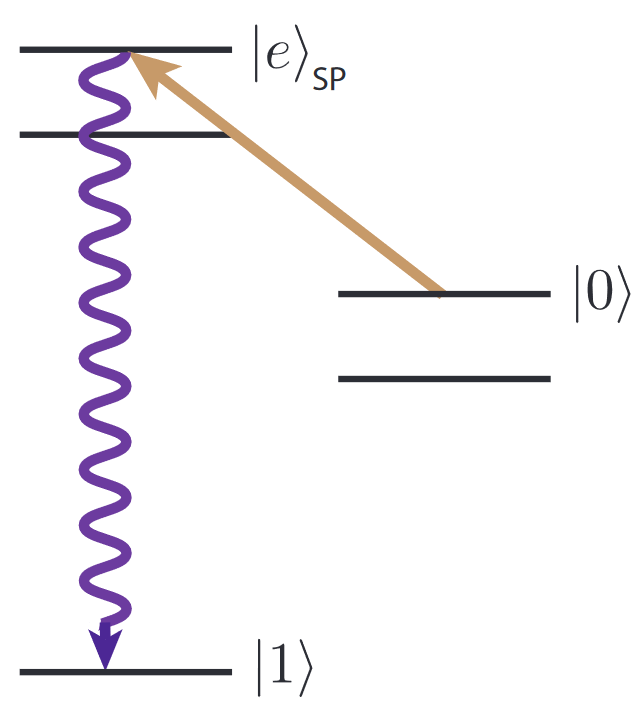
\includegraphics[scale=.30]{images/TrappedIons-StatePreparation.png}
    \caption{Qubit initialization \cite{TrappedIonQuantumComputing_2019}}
    \label{fig:QubitInitialization}
\end{figure}

As shown in figure \ref{fig:QubitReadout}, qubit readout is done by using a resonant laser that couples the $\ket{1}$ state to a $\ket{e}_{R}$ state which scatters many photons that can be collected by a detector. When the ion is in state $\ket{0}$, it does not interact with the laser so no photons are emitted and the image produced by the detector is dark.

\begin{figure}[h!]
    \centering
    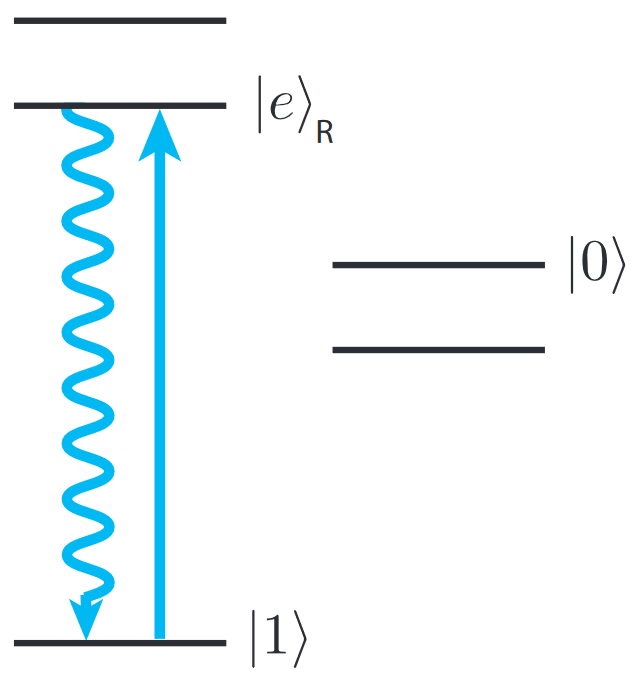
\includegraphics[scale=.25]{images/TrappedIons-QubitReadout.png}
    \caption{Qubit readout \cite{TrappedIonQuantumComputing_2019}}
    \label{fig:QubitReadout}
\end{figure}

A universal gate set is achieved by providing two qubit manipulation mechanisms:
\begin{itemize}[noitemsep,nolistsep]
    \item Arbitrary single qubit rotations: laser or microwave drives applied to the ions allow arbitrary and high fidelity single qubit rotations to be performed.
    \item An entangling operation: motional modes of two or more ions are used as a bus for transfering quantum information among ions.
\end{itemize}

Single qubit gate times are in the order of a few microseconds while two qubit gate times typically take between tens and hundreds of microseconds. Ion coherence times range from 0.2 seconds in optical qubits to up to 600 seconds for hyperfine qubits. Long coherence times relative to gate times fulfill the remaining criteria for a universal quantum computer.

\section{Native Gates}

The native single qubit gate\cite{3QubitGroverSearch_2017} in this physical platform is defined as:
$$R(\theta,\phi)=\left[\begin{array}{cc}\cos{\frac{\theta}{2}} & -\imath e^{-\imath \phi}\sin{\frac{\theta}{2}} \\ -\imath e^{-\imath \phi}\sin{\frac{\theta}{2}} & \cos{\frac{\theta}{2}}\end{array}\right]$$

Rotations about the X-axis ($R_x(\theta)$) are achieved by setting $\phi=0$. Rotations about the Y-axis ($R_y(\theta)$) are achieved by setting $\phi=\frac{\pi}{2}$. Rotations about the Z-axis ($R_z(\theta)$) are achieved by three rotations about axes in the XY plane as shown in figure \ref{fig:RzGate}:

\begin{figure}[h!]
    \centering
    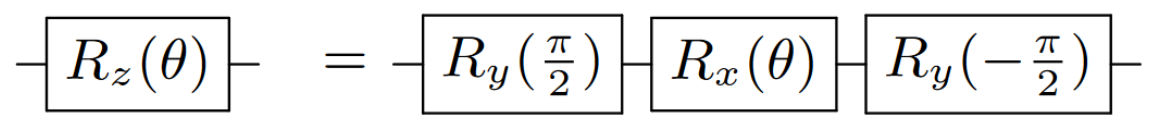
\includegraphics[scale=.35]{images/TrappedIons-RzGate.png}
    \caption{Rz gate \cite{3QubitGroverSearch_2017} decomposition}
    \label{fig:RzGate}
\end{figure}

Note that Pauli gates can be constructed from rotations around the X, Y and Z axis:
\begin{itemize}[noitemsep,nolistsep]
    \item $X=\imath R_x(\pi)$
    \item $Y=\imath R_y(\pi)$
    \item $Z=\imath R_z(\pi)$
\end{itemize}

Another widely used quantum gate is the Hadamard gate, which can be also be decomposed from rotations around the X and Y axis\cite{QuantumInspire_HadamardGate}:
$$H=R_x(\pi)R_y(\frac{\pi}{2})$$

The native two qubit entangling gate\cite{3QubitGroverSearch_2017} in this physical platform is defined as:
$$XX(\chi)=\left[\begin{array}{cccc}\cos{\chi} & 0 & 0 & -\imath\sin{\chi} \\ 0 & \cos{\chi} & -\imath\sin{\chi} & 0 \\ 0 & -\imath\sin{\chi} & cos{\chi} & 0 \\ -\imath\sin{\chi} & 0 & 0 & cos{\chi}\end{array}\right]$$

The CNOT gate, which is more commonly used as an entangling gate when describing quantum algorithms, can be constructed using the $XX(\chi)$ and $R(\theta,\phi)$ gates as shown in figure \ref{fig:CNOTGate}:

\begin{figure}[h!]
    \centering
    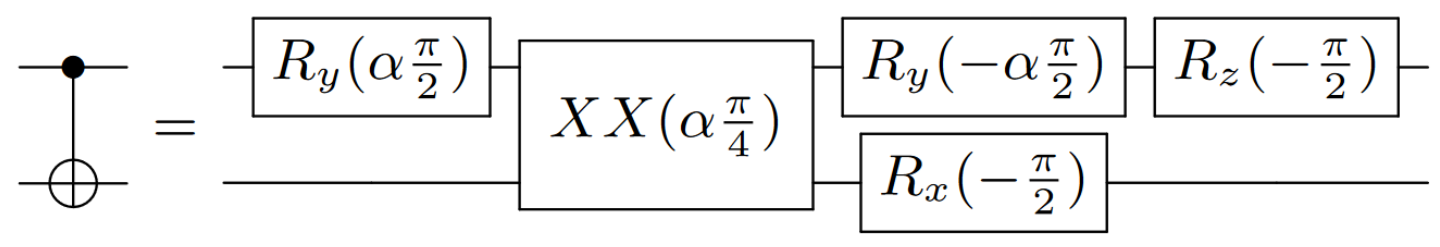
\includegraphics[scale=.35]{images/TrappedIons-CNOTGate.png}
    \caption{CNOT gate \cite{3QubitGroverSearch_2017} decomposition where $\alpha=sgn(\chi)$}
    \label{fig:CNOTGate}
\end{figure}

Using the results demonstrated by C. J. Ballance et al. \cite{TrappedIonHyperfineQubits_2016}, the gate times and fidelities in this physical platform are the following:
\begin{itemize}[noitemsep,nolistsep]
    \item Single qubit arbitrary rotation gate ($R(\theta,\phi)$):
    \begin{itemize}[noitemsep,nolistsep]
        \item Time: 7.5 $\mu s$
        \item Fidelity: 0.99993
    \end{itemize}
    \item Two qubit entangling gate ($XX(\chi)$): .
    \begin{itemize}[noitemsep,nolistsep]
        \item Time: 100 $\mu s$
        \item Fidelity: 0.999
    \end{itemize}
\end{itemize}

Additionally, we will consider qubit readout (measurement) to be perfomed in 400 $\mu s$\cite{TrappedIonQuantumComputing_2019}.

\section{Resources Estimation Analysis}

We customized the trace simulator included in Microsoft's Quantum Development Kit to use specific gate times to calculate the depth of the circuit. More specifically, we used the following gate times configuration (based on the characteristics presented earlier in this chapter):
\begin{itemize}
    \item R gate: 7.5 $\mu s$
    \item T gate: 7.5 $\mu s$
    \item Clifford gates: 7.5 $\mu s$
    \item CNOT gate: 122.5 $\mu s$
    \item Measurement gate (qubit readout): 400 $\mu s$
\end{itemize}

A sample of an execution of the console application using the $trackionresources$ command is shown in listing \ref{lst:TrackIonResourcesOutput}.

\begin{lstlisting}[label=lst:TrackIonResourcesOutput,caption={Output of tracking Ion platform resources for Shor's algorithm}]
> dotnet run -- trackionresources -N 15 --generator 11
Gate times configuration:
CNOT: 122.5
Measure: 400
QubitClifford: 7.5
R: 7.5
T: 7.5

Depth: 5.10198 seconds.
Width: 21 qubits.
\end{lstlisting}

\section{Analysis of Execution in NISQ Devices}

Running the tool multiple times and collecting the data it produced, we can see that for a NISQ device we could factorize a 20-bit semiprime integer using 85 quibits. This does not take into account error correction so this might not be realistic since we might not be confident about the computation result.

\begin{figure}[h!]
    \centering
    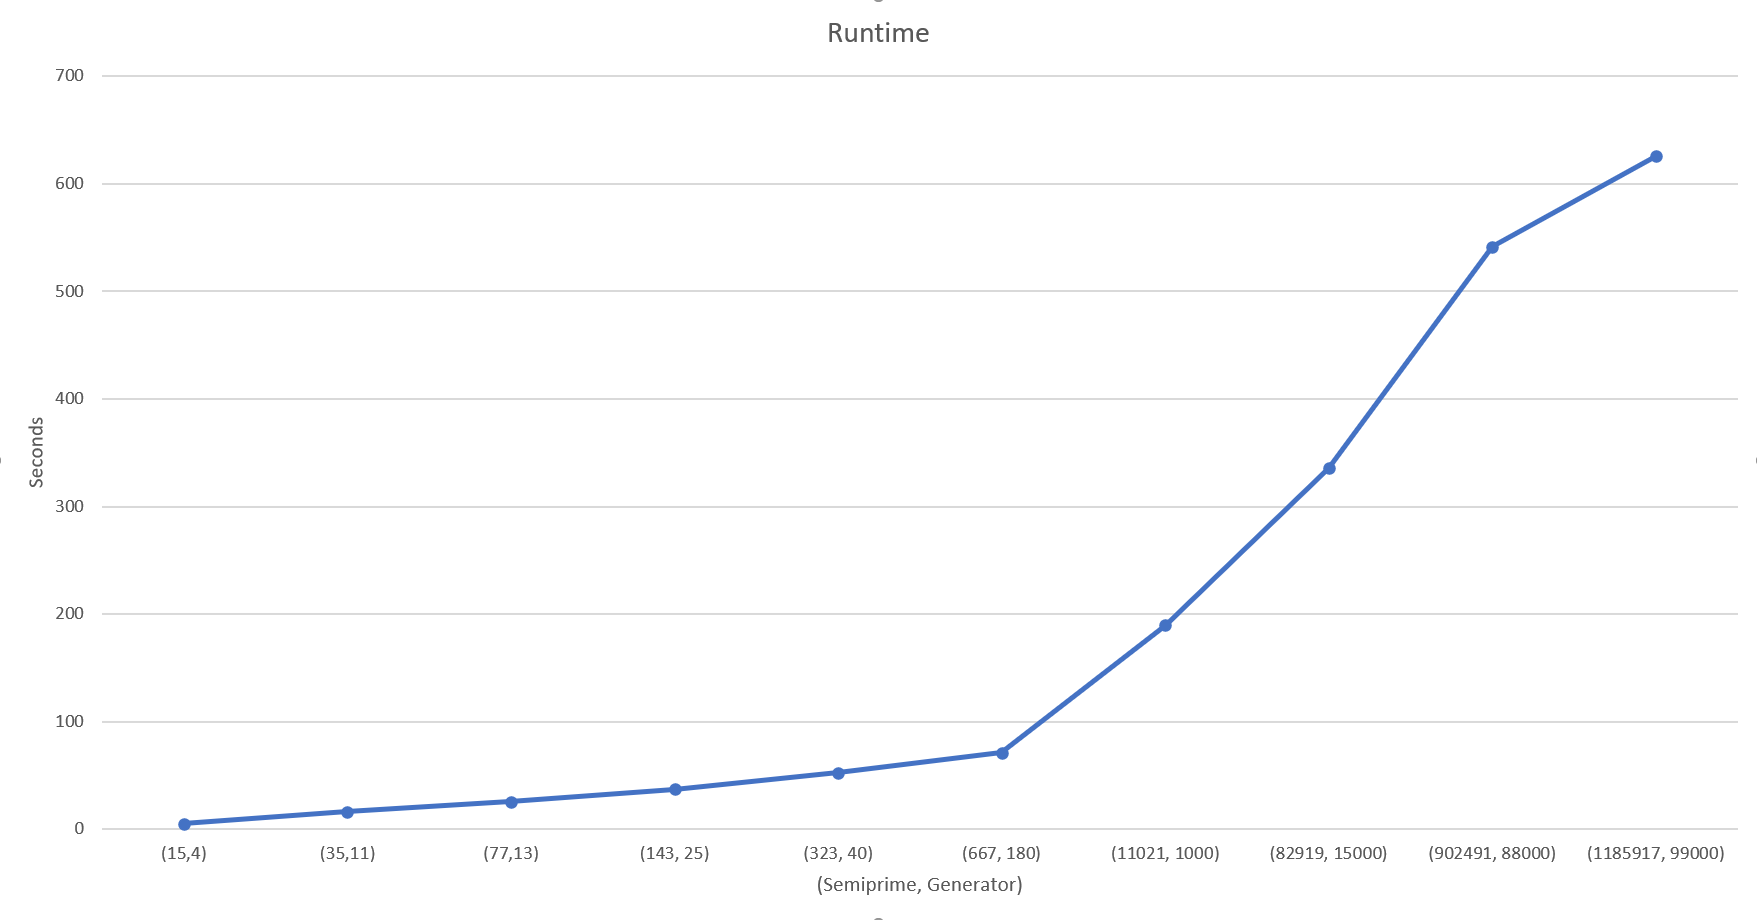
\includegraphics[scale=.35]{images/TrappedIons-NisqRuntime.png}
    \caption{NISQ Runtime}
    \label{fig:NisqRuntime}
\end{figure}

%
% Chapter 9
%
\chapter {Superconducting Physical Platform}

\todo{Briefly describe this quantum computing platform.}

\section{Native Gates and Platform Characteristics}

\todo{Enumerate the native gates that this platform implements, its characteristics (fidelity, gate time), and how logical gates are implemented (using circuits to illustrate them).}

\section{Resources Estimation Analysis}

\todo{Show (using tables and/or plots) how resources escalate as the size and pattern of the input changes}.

\section{Analysis of Execution in NISQ Devices}

\todo{Analyze what would be the maximum input size that can be successfully run on a NISQ device based on this platform.}

\section{Analysis of Execution of Algorithm for Input of Specific Size}

\todo{Use a resource estimator to determine the characteristics that a device should have to run the algorithm for a specific input size, and determine what would be the runtime.}



%
% Chapter 10
%
\chapter {Physical Platforms Comparison}

\todo{Compare the results obtained from both hardware platforms and comment on the insights obtained.}
%
% Chapter 11
%
\chapter {Future Work}

\todo{Mention how this framework can be used to analyze and compare other hardware platforms.}


%
% Bibliography
%
\bibliographystyle{plain}
\bibliography{thesis}

%
% Appendices
%
\appendix
%
% Appendix A
%
\chapter{Implementation of Generic Physical Resources Estimation Framework}

\todo{Add source code that implements the physical resources estimation framework.}

Source code can also be found in \href{https://github.com/cesarzc/qc-resources-estimation}{GitHub}.


\end{document}
